% Options for packages loaded elsewhere
\PassOptionsToPackage{unicode}{hyperref}
\PassOptionsToPackage{hyphens}{url}
%
\documentclass[
]{book}
\usepackage{amsmath,amssymb}
\usepackage{iftex}
\ifPDFTeX
  \usepackage[T1]{fontenc}
  \usepackage[utf8]{inputenc}
  \usepackage{textcomp} % provide euro and other symbols
\else % if luatex or xetex
  \usepackage{unicode-math} % this also loads fontspec
  \defaultfontfeatures{Scale=MatchLowercase}
  \defaultfontfeatures[\rmfamily]{Ligatures=TeX,Scale=1}
\fi
\usepackage{lmodern}
\ifPDFTeX\else
  % xetex/luatex font selection
\fi
% Use upquote if available, for straight quotes in verbatim environments
\IfFileExists{upquote.sty}{\usepackage{upquote}}{}
\IfFileExists{microtype.sty}{% use microtype if available
  \usepackage[]{microtype}
  \UseMicrotypeSet[protrusion]{basicmath} % disable protrusion for tt fonts
}{}
\makeatletter
\@ifundefined{KOMAClassName}{% if non-KOMA class
  \IfFileExists{parskip.sty}{%
    \usepackage{parskip}
  }{% else
    \setlength{\parindent}{0pt}
    \setlength{\parskip}{6pt plus 2pt minus 1pt}}
}{% if KOMA class
  \KOMAoptions{parskip=half}}
\makeatother
\usepackage{xcolor}
\usepackage{longtable,booktabs,array}
\usepackage{calc} % for calculating minipage widths
% Correct order of tables after \paragraph or \subparagraph
\usepackage{etoolbox}
\makeatletter
\patchcmd\longtable{\par}{\if@noskipsec\mbox{}\fi\par}{}{}
\makeatother
% Allow footnotes in longtable head/foot
\IfFileExists{footnotehyper.sty}{\usepackage{footnotehyper}}{\usepackage{footnote}}
\makesavenoteenv{longtable}
\usepackage{graphicx}
\makeatletter
\def\maxwidth{\ifdim\Gin@nat@width>\linewidth\linewidth\else\Gin@nat@width\fi}
\def\maxheight{\ifdim\Gin@nat@height>\textheight\textheight\else\Gin@nat@height\fi}
\makeatother
% Scale images if necessary, so that they will not overflow the page
% margins by default, and it is still possible to overwrite the defaults
% using explicit options in \includegraphics[width, height, ...]{}
\setkeys{Gin}{width=\maxwidth,height=\maxheight,keepaspectratio}
% Set default figure placement to htbp
\makeatletter
\def\fps@figure{htbp}
\makeatother
\setlength{\emergencystretch}{3em} % prevent overfull lines
\providecommand{\tightlist}{%
  \setlength{\itemsep}{0pt}\setlength{\parskip}{0pt}}
\setcounter{secnumdepth}{5}
\usepackage{booktabs}
\usepackage{amsthm}
\makeatletter
\def\thm@space@setup{%
  \thm@preskip=8pt plus 2pt minus 4pt
  \thm@postskip=\thm@preskip
}
\makeatother
\ifLuaTeX
  \usepackage{selnolig}  % disable illegal ligatures
\fi
\usepackage[]{natbib}
\bibliographystyle{apalike}
\usepackage{bookmark}
\IfFileExists{xurl.sty}{\usepackage{xurl}}{} % add URL line breaks if available
\urlstyle{same}
\hypersetup{
  pdftitle={Manual de usuario de MonitorEO-EarthCul.},
  pdfauthor={EarthCul PID2020-118041GB-I00.},
  hidelinks,
  pdfcreator={LaTeX via pandoc}}

\title{Manual de usuario de MonitorEO-EarthCul.}
\author{EarthCul PID2020-118041GB-I00.}
\date{2025-04-23}

\begin{document}
\maketitle

{
\setcounter{tocdepth}{1}
\tableofcontents
}
\chapter{Introducción}\label{intro}

MonitorEO-EarthCul es una herramienta de análisis de variables derivadas de teledetección satelital basada en Google Earth Engine desarrollada por proyecto EarthCul PID2020-118041GB-I00.

Este manual de usuario proporciona una guía completa para el uso de MonitorEO-EarthCul, incluyendo la descripción de funcionalidades, navegación por la interfaz, selección de parámetros y visualización de resultados.

Este proyecto ha sido financiado por el Ministerio de Ciencia e Innovación


\includegraphics{assets/logo-ugr.png}

\chapter{Interfaz de MonitorEO-EarthCul}\label{interfaz}

La interfaz gráfica del \textbf{Laboratorio de Investigación Virtual MonitorEO-EarthCul} (\emph{Monitoring with Earth Observations} del \textbf{Proyecto EarthCul PID2020-118041GB-I00}) ha sido diseñado para la observación de \textbf{servicios ecosistémicos culturales}. La interfaz permite la exploración espacial y temporal de las cartografías generadas por el proyecto en diferentes áreas protegidas de montaña.

MonitorEO-EarthCul integra colecciones de datos satelitales, herramientas de análisis geoespacial y una interfaz interactiva que facilita su uso tanto en estudios científicos como en aplicaciones de gestión.

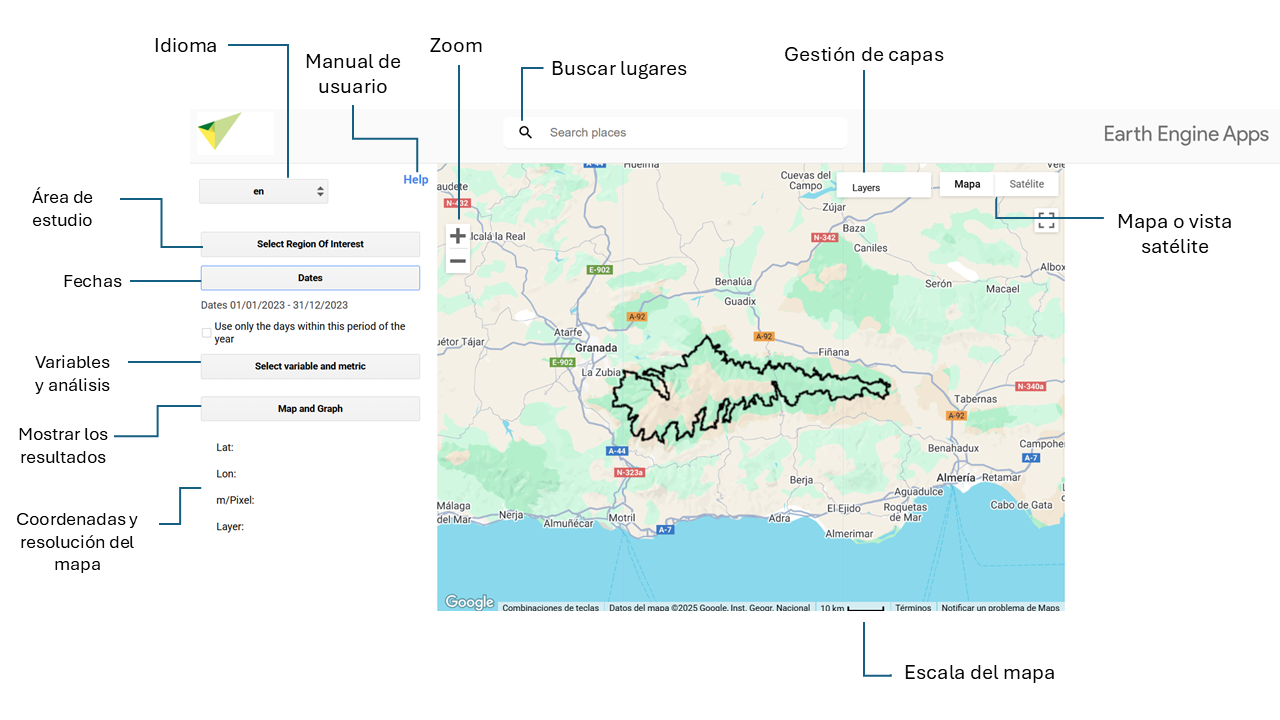
\includegraphics{assets/InterfazMonitorEO_es.png}

\chapter{Idiomas}\label{idiomas}

🌐 Selecciona el idioma de la interfaz. Están disponibles las siguientes opciones:

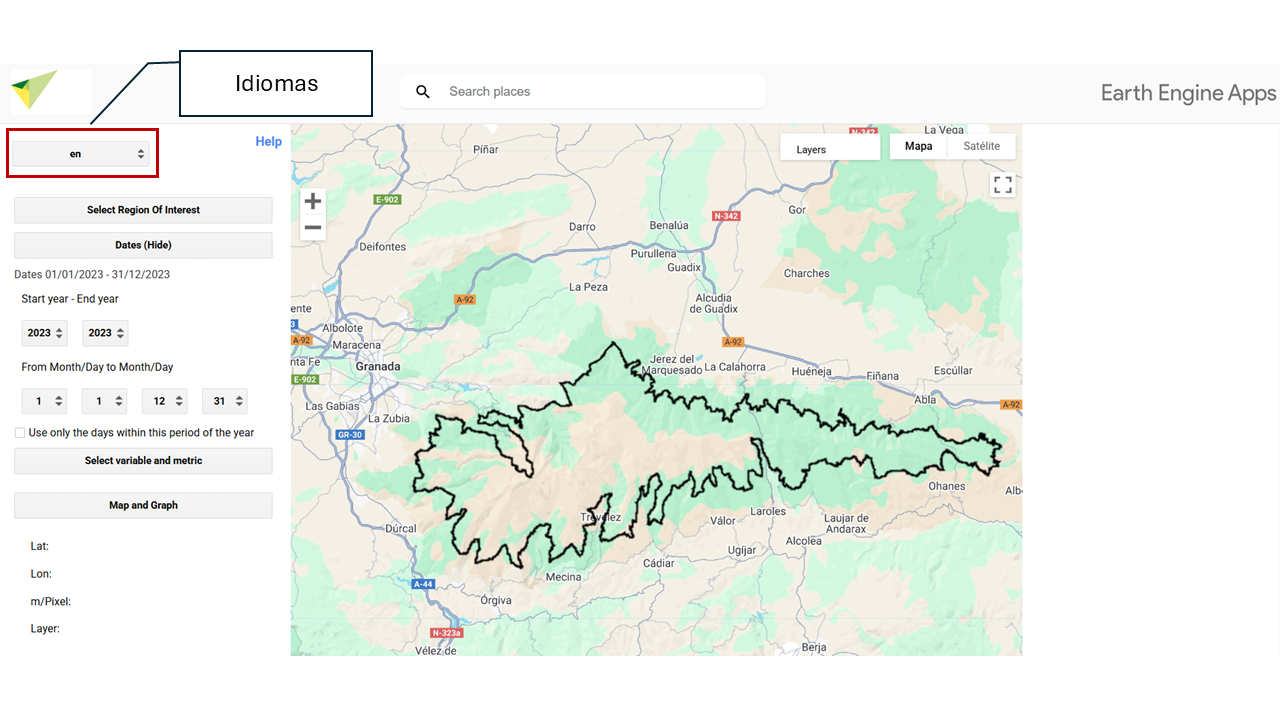
\includegraphics{assets/Idiomas.png}

\begin{itemize}
\item
  \textbf{es}
  Español
\item
  \textbf{en}
  English
\item
  \textbf{fr}
  Français
\item
  \textbf{de}
  Deutsch
\end{itemize}

\chapter{Área de estudio}\label{area-estudio}

\textbf{Selecciona ROI-- Elige tu área de estudio.}

En esta sección puedes definir la \textbf{región de interés (ROI)} sobre la que se realizará el análisis. Tienes varias opciones disponibles para seleccionar o cargar tu área de estudio.

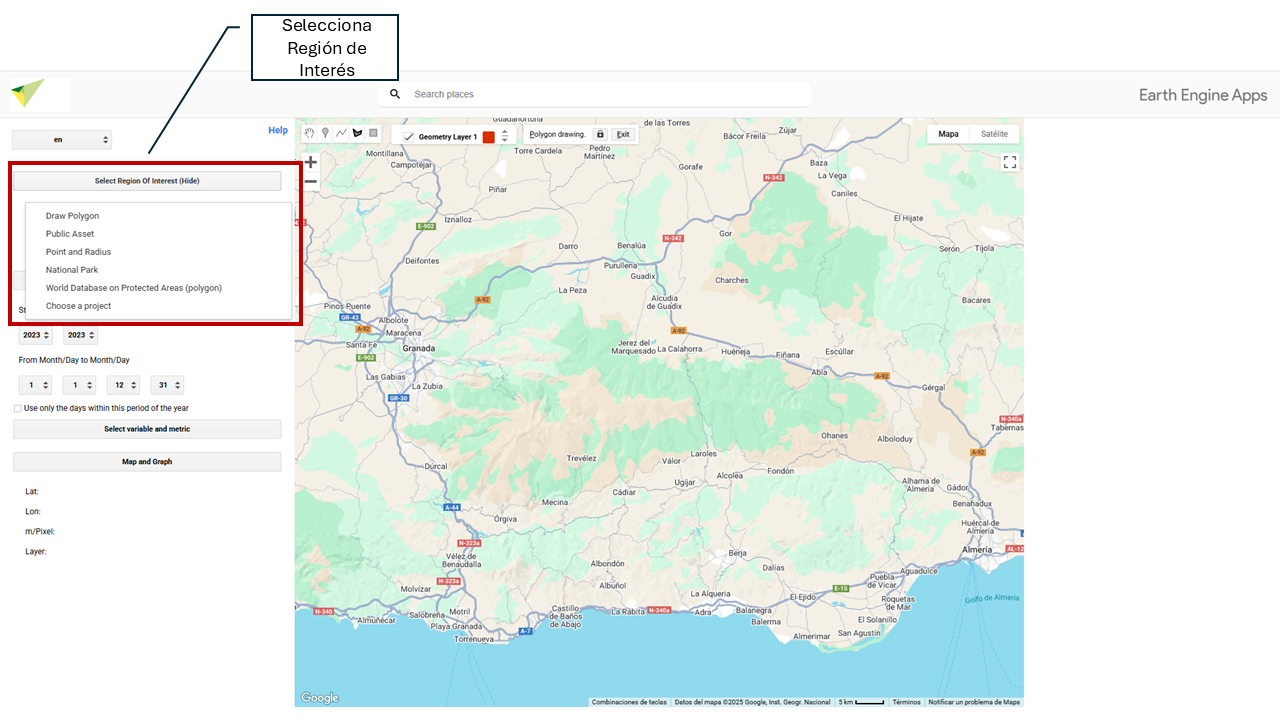
\includegraphics{assets/ROI_es.png}

\section{\texorpdfstring{\textbf{🏞️ Parque Nacional EarthCul}}{🏞️ Parque Nacional EarthCul}}\label{parque-nacional-earthcul}

Puedes seleccionar como área de estudio cualquiera de los \textbf{Parques Nacionales de España y Portugal} disponibles en la plataforma.

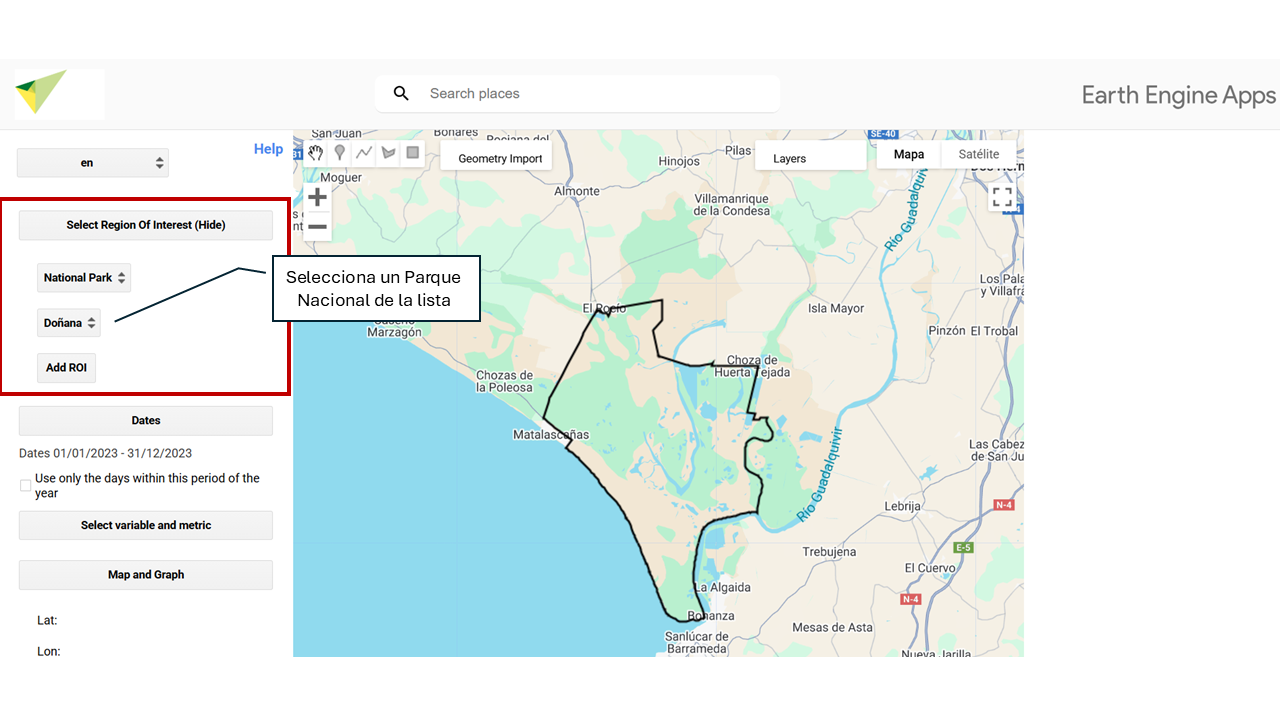
\includegraphics{assets/np_es.png}

\section{\texorpdfstring{\textbf{📁 Área de influencia socioeconómica parques EarthCul}}{📁 Área de influencia socioeconómica parques EarthCul}}\label{uxe1rea-de-influencia-socioeconuxf3mica-parques-earthcul}

Puedes seleccionar como área de estudio las zonas asociadas al proyecto:

\begin{itemize}
\tightlist
\item
  \textbf{EarthCul}: Áreas de influencia socioeconómica de los Parques Nacionales de montaña en España y Portugal.
\end{itemize}

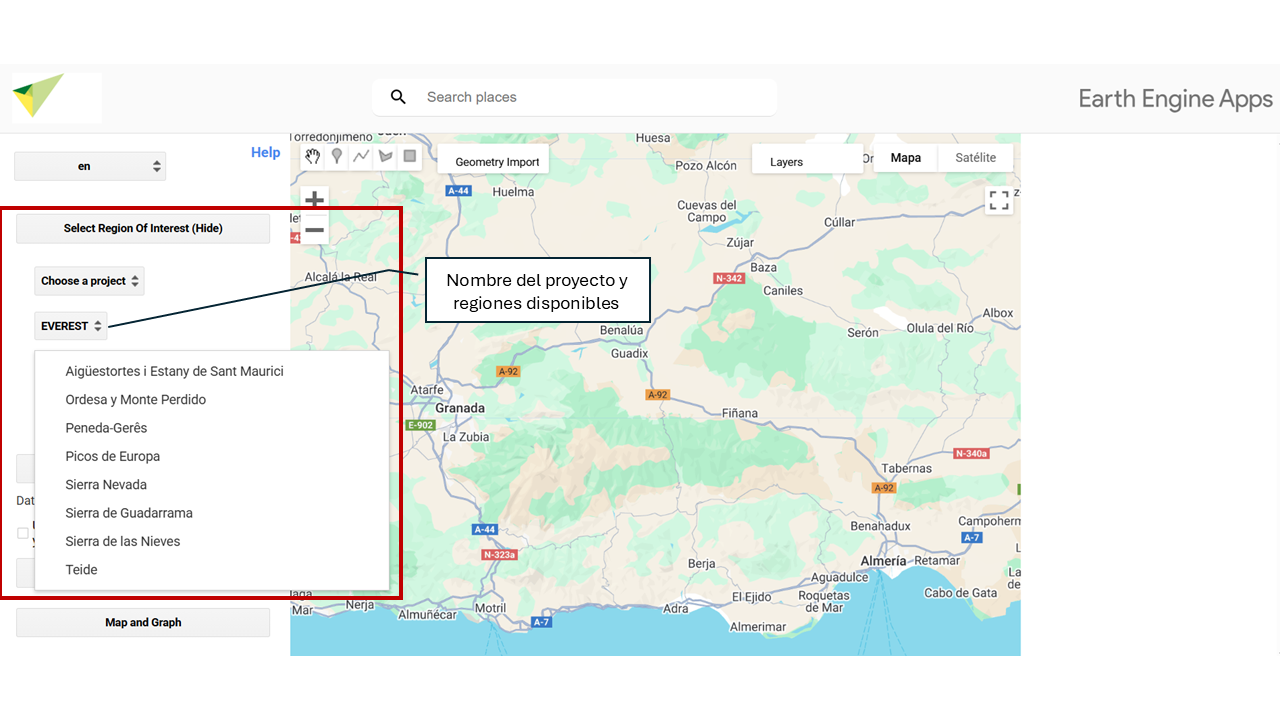
\includegraphics{assets/PROJECTS_es.png}

\chapter{Fechas de inicio y fin}\label{fechas}

Elige el rango de fechas para realizar tus cálculos. Primero, establece el \textbf{año de inicio} y el \textbf{año de fin}. Luego, selecciona el \textbf{mes y día de inicio}, así como el \textbf{mes y día de finalización} para definir el período de análisis.

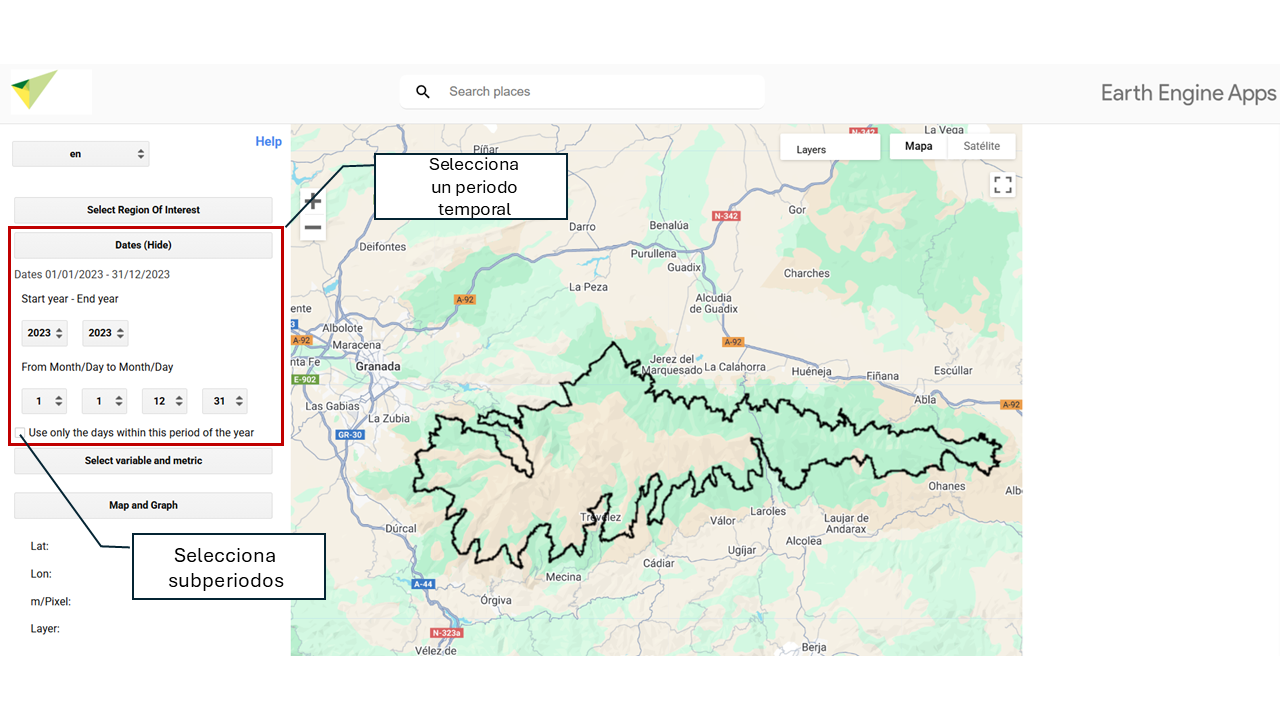
\includegraphics{assets/dates_es.png}

\section{\texorpdfstring{\textbf{📆Selección de un intervalo específico}}{📆Selección de un intervalo específico}}\label{selecciuxf3n-de-un-intervalo-especuxedfico}

La herramienta permite seleccionar un \textbf{intervalo específico dentro del año} para realizar un análisis estacional.

Al activar la opción \textbf{``Utilice solo los días de este periodo del año''}, se delimita un rango de fechas (por ejemplo, del \textbf{21 de marzo al 21 de septiembre)} que se aplicará a \textbf{cada año} del periodo seleccionado (por ejemplo, de 2001 a 2020).

Esto permite analizar únicamente ciertos meses o estaciones, como \textbf{primaveras, veranos, o estaciones de crecimiento.}

Si seleccionas:

\begin{itemize}
\tightlist
\item
  Año inicio: 2001\\
\item
  Año fin: 2020\\
\item
  Desde: 21/03\\
\item
  Hasta: 21/09
\end{itemize}

Se analizarán sólo los días comprendidos entre el 21 de marzo y el 21 de septiembre en cada uno de esos años, excluyendo el resto.

\chapter{Tipo de variable de interés}\label{tipo-variable}

Selecciona la variable de estudio. Las variables se clasifican en grandes categorías de \href{https://geobon.org/ebvs/what-are-ebvs/}{EBVs} \{target=\_blank\} \textbf{(Variables Esenciales de Biodiversidad)}, relacionadas con el funcionamiento y estructura de los ecosistemas. \textbf{MonitorEO-OBSNEV} incluye:

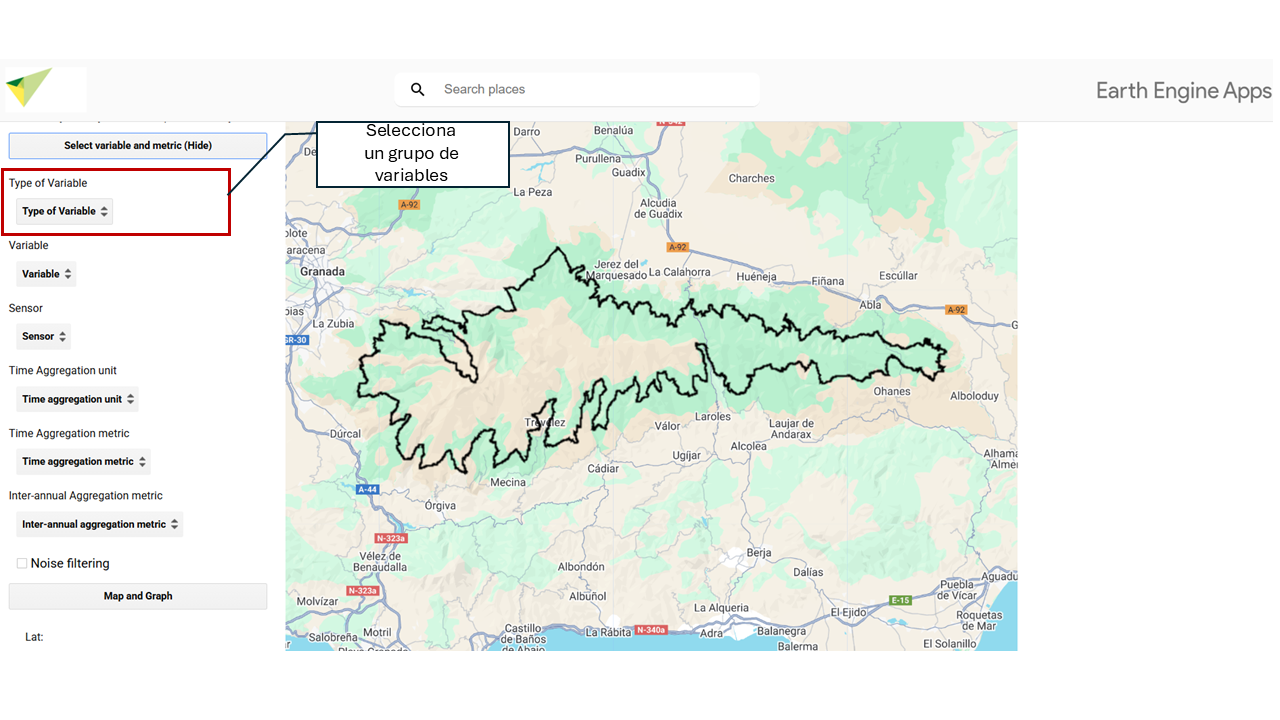
\includegraphics{assets/variables_es.png}

\section{\texorpdfstring{\textbf{🌱 Carbono Orgánico (Producción Primaria)}}{🌱 Carbono Orgánico (Producción Primaria)}}\label{carbono-orguxe1nico-producciuxf3n-primaria}

\subsection{\texorpdfstring{\textbf{NDVI} - Índice de Vegetación de Diferencia Normalizada}{NDVI - Índice de Vegetación de Diferencia Normalizada}}\label{ndvi---uxedndice-de-vegetaciuxf3n-de-diferencia-normalizada}

El Índice de Vegetación de Diferencia Normalizada (NDVI, por sus siglas en inglés) es un indicador espectral ampliamente utilizado para cuantificar la cobertura y el estado de la vegetación mediante sensores remotos. Se calcula a partir de la diferencia entre la reflectancia en el infrarrojo cercano (NIR) y la reflectancia en el rojo (RED), normalizada por su suma:

NDV I= NIR- RED / NIR + RED

Este índice toma valores entre -1 y 1. Valores cercanos a 1 indican vegetación densa y vigorosa, mientras que valores cercanos a -1 corresponden a superficies no vegetadas, como cuerpos de agua, nieve o áreas urbanas.

Unidades: sin unidad.

\subsection{\texorpdfstring{\textbf{EVI} - Índice de Vegetación Mejorado}{EVI - Índice de Vegetación Mejorado}}\label{evi---uxedndice-de-vegetaciuxf3n-mejorado}

El Índice de Vegetación Mejorado (EVI, por sus siglas en inglés) es un indicador espectral desarrollado para optimizar la estimación de la cobertura y condición de la vegetación a partir de datos de teledetección. A diferencia de índices tradicionales como el NDVI, el EVI incorpora factores de corrección atmosférica y una compensación por la influencia del fondo del suelo, lo que mejora su sensibilidad en áreas con alta densidad de vegetación, baja cobertura vegetal o condiciones atmosféricas complejas.

La fórmula general del EVI es la siguiente:

EVI=G⋅ NIR−RED / NIR+C1\hspace{0pt}⋅RED−C2\hspace{0pt}⋅BLUE+L

donde:

\begin{itemize}
\tightlist
\item
  NIR: reflectancia en el infrarrojo cercano\\
\item
  RED: reflectancia en el rojo\\
\item
  BLUE: reflectancia en el azul\\
\item
  G: factor de ganancia (generalmente 2.5)\\
\item
  L: factor de corrección del suelo (1.0)\\
\item
  C1 y C2\hspace{0pt}: coeficientes de corrección atmosférica (6.0 y 7.5, respectivamente)
\end{itemize}

Los valores del EVI varían entre -1 y 1. Valores cercanos a 1 indican una vegetación densa y saludable, mientras que valores negativos o bajos reflejan áreas sin vegetación, como cuerpos de agua, zonas urbanizadas o superficies nevadas.

\begin{longtable}[]{@{}
  >{\raggedright\arraybackslash}p{(\columnwidth - 2\tabcolsep) * \real{0.5000}}
  >{\centering\arraybackslash}p{(\columnwidth - 2\tabcolsep) * \real{0.5000}}@{}}
\toprule\noalign{}
\begin{minipage}[b]{\linewidth}\raggedright
Valor de EVI
\end{minipage} & \begin{minipage}[b]{\linewidth}\centering
Interpretación ecológica
\end{minipage} \\
\midrule\noalign{}
\endhead
\bottomrule\noalign{}
\endlastfoot
\textbf{\textless{} 0.0} & Agua, nieve, nubes, áreas no vegetadas \\
\textbf{0.0 -- 0.1} & Suelos desnudos, desiertos, áreas urbanas, rocas \\
\textbf{0.1 -- 0.2} & Vegetación escasa, pastizales áridos, matorral abierto \\
\textbf{0.2 -- 0.3} & Pastizales, agricultura de secano, sabanas \\
\textbf{0.3 -- 0.5} & Bosques abiertos, zonas agrícolas activas (cultivos en crecimiento) \\
\textbf{0.5 -- 0.7} & Bosques templados densos, cultivos con alta cobertura vegetal \\
\textbf{\textgreater{} 0.7} & Bosques tropicales, selvas, vegetación muy densa \\
\end{longtable}

Unidades: sin unidad.

\subsection{\texorpdfstring{\textbf{Chl-a} - Concentración de clorofila}{Chl-a - Concentración de clorofila}}\label{chl-a---concentraciuxf3n-de-clorofila}

El índice de clorofila-a se utiliza para estimar la concentración de clorofila-a en cuerpos de agua como océanos, lagos y ríos. La clorofila-a es el principal pigmento fotosintético presente en el fitoplancton, por lo que su concentración actúa como un indicador indirecto de la biomasa algal y de la productividad primaria en ecosistemas acuáticos, siendo un indicador clave para evaluar la calidad del agua y la salud de los ecosistemas acuáticos (Gitelson et al., 1993; IOCCG, 2000).

Unidades: mg m-3.

\section{\texorpdfstring{\textbf{🌞 Balance de Radiación}}{🌞 Balance de Radiación}}\label{balance-de-radiaciuxf3n}

\subsection{\texorpdfstring{\textbf{ALB} - Albedo}{ALB - Albedo}}\label{alb---albedo}

El albedo es la fracción de la radiación solar incidente que es reflejada por una superficie sin ser absorbida. Se trata de un parámetro adimensional que varía entre 0 (absorción total) y 1 (reflexión total). Un albedo elevado indica que la superficie refleja una gran proporción de la energía solar recibida, como ocurre en superficies altamente reflectantes como la nieve o el hielo. En contraste, un albedo bajo implica una mayor absorción de radiación, característica de superficies oscuras como áreas urbanas, suelos húmedos o cuerpos de agua.\\
El albedo desempeña un papel clave en el balance energético terrestre y en procesos relacionados con el clima global, ya que influye directamente en la cantidad de energía que entra y se retiene en el sistema climático.

Unidades: sin unidad.

\section{\texorpdfstring{\textbf{💧Balance de Agua}}{💧Balance de Agua}}\label{balance-de-agua}

\subsection{\texorpdfstring{\textbf{ET} - Evapotranspiración}{ET - Evapotranspiración}}\label{et---evapotranspiraciuxf3n}

Estimación de la cantidad de agua que se evapora de la superficie terrestre y se transpira por las plantas. Generada a partir del modelo Mu et al.~(2011), que implementa un enfoque basado en la ecuación de Penman-Monteith, adaptada para sensores remotos. Permite comprender el ciclo del agua, evaluar la disponibilidad de agua en una región y monitorear los recursos hídricos.

Unidades: Kj/m\^{}2/8days

\subsection{\texorpdfstring{\textbf{LE} - Calor Latente}{LE - Calor Latente}}\label{le---calor-latente}

Estimación indirecta de la energía consumida por la evapotranspiración. Durante el proceso, se requiere energía para romper o formar enlaces entre las moléculas de la sustancia, lo que resulta en la liberación o absorción de calor. El calor latente desempeña un papel fundamental en el ciclo del agua, ya que la evaporación y la condensación son procesos clave en la formación de nubes, la precipitación y la regulación del clima.

Unidades: J/m\^{}2/day

\subsection{\texorpdfstring{\textbf{LSWI} - Índice de Agua Superficial Terrestre}{LSWI - Índice de Agua Superficial Terrestre}}\label{lswi---uxedndice-de-agua-superficial-terrestre}

El LSWI (Land Surface Water Index) es un índice espectral utilizado para detectar y evaluar la presencia de humedad en la superficie terrestre, particularmente en la vegetación y el suelo. Se basa en la diferencia entre la reflectancia en el infrarrojo cercano (NIR) y el infrarrojo de onda corta (SWIR), que son sensibles al contenido de agua en la vegetación y el suelo.

LSWI = NIR- SWIR / NIR + SWIR\hspace{0pt}

\begin{itemize}
\item
  NIR: Banda de infrarrojo cercano.
\item
  SWIR: Banda de infrarrojo de onda corta.
\end{itemize}

\textbf{Valores altos} → alta humedad superficial, suelos húmedos, vegetación con alto contenido de agua, humedales o áreas agrícolas irrigadas.

\textbf{Valores bajos} → condiciones secas, vegetación estresada o suelos áridos.

Unidades: sin unidad.

\subsection{\texorpdfstring{\textbf{NDWI} - Índice de Agua de Diferencia Normalizada}{NDWI - Índice de Agua de Diferencia Normalizada}}\label{ndwi---uxedndice-de-agua-de-diferencia-normalizada}

El NDWI ( Normalized Difference Water Index) es un índice espectral diseñado para detectar y cuantificar la presencia de agua en la superficie terrestre. Se basa en la diferencia de reflectancia entre el infrarrojo cercano (NIR) y el verde (Green), aprovechando la fuerte absorción del agua en el NIR y su alta reflectancia en el visible.

NDWI = Green - NIR / Green + NIR\hspace{0pt}

\begin{itemize}
\tightlist
\item
  Green: Banda del verde.\\
\item
  NIR: Banda del infrarrojo cercano
\end{itemize}

\textbf{NDWI \textgreater{} 0} → presencia de \textbf{agua superficial} (ríos, lagos, embalses, zonas inundadas)\\
\textbf{NDWI \textless{} 0} → superficies \textbf{terrestres sin agua} (vegetación, suelo desnudo, áreas urbanas)

Unidades: sin unidad.

\subsection{\texorpdfstring{\textbf{NDSI} - Índice de Nieve de Diferencia Normalizada}{NDSI - Índice de Nieve de Diferencia Normalizada}}\label{ndsi---uxedndice-de-nieve-de-diferencia-normalizada}

El NDSI ( Normalized Difference Snow Index) es un indicador espectral utilizado para detectar la presencia y extensión de nieve en la superficie terrestre. Se basa en las características reflectivas distintivas de la nieve, que refleja fuertemente en el espectro visible (banda verde) y absorbe significativamente en el infrarrojo de onda corta (SWIR), en contraste con la mayoría de los demás tipos de cobertura terrestre.

NDSI = Green - SWIR / Green + SWIR\hspace{0pt}

\begin{itemize}
\tightlist
\item
  \textbf{Green}: Banda del verde.\\
\item
  \textbf{SWIR}: Banda del infrarrojo de onda corta.
\end{itemize}

\textbf{NDSI \textgreater{} 0.4} → alta probabilidad de presencia de \textbf{nieve o hielo.}\\
\textbf{NDSI \textless{} 0.2} → generalmente indica \textbf{ausencia de nieve.}

Estos umbrales pueden ajustarse según la resolución y el sensor utilizado.

Unidades: sin unidad.

\section{\texorpdfstring{\textbf{🌡️ Calor Sensible}}{🌡️ Calor Sensible}}\label{calor-sensible}

\subsection{\texorpdfstring{\textbf{LST} -Temperatura Superficial}{LST -Temperatura Superficial}}\label{lst--temperatura-superficial}

La temperatura de la superficie terrestre (LST, por sus siglas en inglés) se refiere a la temperatura registrada en la capa superior de la superficie terrestre o de los cuerpos de agua, tal como es detectada por sensores remotos. LST se estima a partir de la radiancia térmica captada en el espectro del infrarrojo térmico, y es una variable clave en el análisis de procesos como el balance energético, la evapotranspiración, la sequía, el estrés hídrico y el monitoreo urbano y agrícola.

Unidades: ºC.

\section{\texorpdfstring{\textbf{💨 Nutrientes / Aerosoles}}{💨 Nutrientes / Aerosoles}}\label{nutrientes-aerosoles}

\subsection{\texorpdfstring{\textbf{ARSL} - Profundidad óptica atmosférica de aerosoles}{ARSL - Profundidad óptica atmosférica de aerosoles}}\label{arsl---profundidad-uxf3ptica-atmosfuxe9rica-de-aerosoles}

Cantidad de aerosoles en la columna total atmosférica. Sirve para cuantificar cuánta carga de aerosoles hay en la atmósfera. El espesor óptico total de los aerosoles se refiere a todos los tipos de aerosol mientras que algunos productos de satélite dan información sobre el espesor óptico de un tipo de aerosol en concreto, como por ejemplo, el espesor óptico debido al polvo, que cuantifica la carga de polvo en la columna atmosférica.

Unidades: sin unidad.

\chapter{Sensor satelital}\label{sensor}

Selecciona con qué sensor quieres trabajar. Los sensores disponibles poseen distinta resolución temporal y espacial. Dependiendo de la variable elegida, obtendrás disponibilidad de datos para unos u otros sensores.

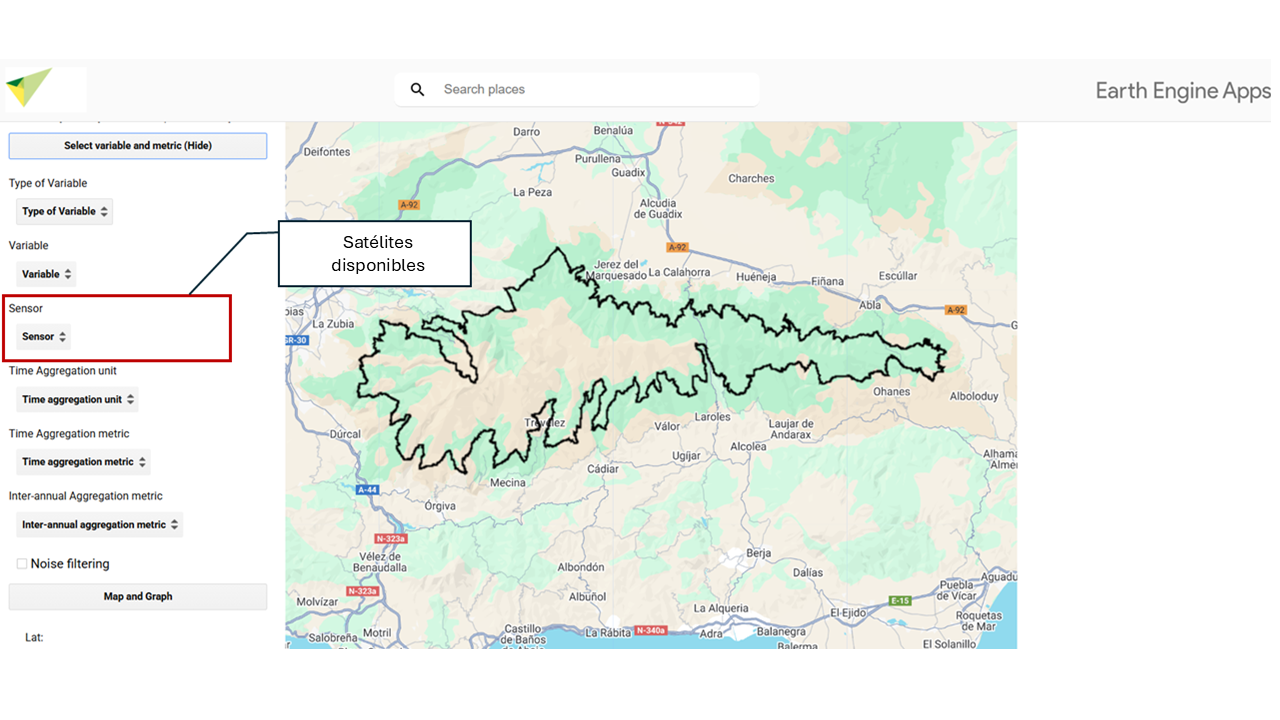
\includegraphics{assets/sensor_es.png}

\textbf{🛰️MODIS 250 m, 16 días}

MODIS (\emph{Moderate Resolution Imaging Spectroradiometer}) es un sensor a bordo de los satélites Terra y Aqua de la NASA.

\textbf{Resolución espacial:} Depende de la variable seleccionada. Pueden ser datos a 250m, 1km, 4km\ldots{} Esta información te aparecerá en la pestaña ``Sensor'' una vez hayas seleccionado tu variable.
\textbf{Resolución temporal:} Depende de la variable seleccionada. Pueden ser datos diarios, cada 8 días o cada 16 días. Esta información te aparecerá en la pestaña ``Sensor'' una vez hayas seleccionado tu variable.

Para esta interfaz, se han utilizado los datos de las colecciones \textbf{MODIS Terra}.

Estos satélites \textbf{proporcionan datos desde} el \textbf{24/02/2000 hasta la actualidad}, aunque la disponibilidad puede variar según la variable seleccionada.

\textbf{🛰️Landsat 30 m, \textgreater{} 16 días}

La serie \textbf{Landsat} es operada por la NASA y el USGS. Estos datos incluyen Landsat 5, 7, 8 y 9.

\textbf{Resolución espacial:} 30 metros.
\textbf{Resolución temporal:} Mayor a 16 días, ya que dependiendo del satélite tienen un período de revisita de 8 o 16 días cada uno.

El \textbf{rango de fechas} cubierto va desde \textbf{1984 hasta la actualidad}, dependiendo de la disponibilidad de cada satélite:
\textbf{Landsat 5} (16/03/1984 - 05/05/2012)
\textbf{Landsat 7} (28/05/1999 - actualidad, con limitaciones desde 31/05/2003 por la falla del ETM+)
\textbf{Landsat 8} (18/03/2013 - presente)
\textbf{Landsat 9} (31/10/2021 - presente)

Entre el \textbf{05/05/2012 y el 18/03/2013}, no hay datos disponibles debido a la interrupción en la captura de imágenes de Landsat 7. Aunque este satélite siguió operando, su utilidad estaba limitada desde 2003 por una falla en el Escáner de Línea de Mejora (ETM+). Debido a esta limitación, a partir de 2003 sus datos no se consideran en el rango completo de fechas disponibles.

\textbf{🛰️Sentinel-2 10m, 5 días}

El programa \textbf{Sentinel-2} es operado por la Agencia Espacial Europea (ESA) y forma parte del programa Copernicus.

\textbf{Resolución espacial:} 10 metros.
\textbf{Resolución temporal:} 5 días.

En esta interfaz, utilizamos el producto \textbf{SR Harmonized}, un producto de Reflectancia de Superficie (SR) ajustado para garantizar la coherencia entre los sensores de Sentinel-2A y Sentinel-2B mediante corrección atmosférica, ajuste espectral y normalización de datos.

El \textbf{rango de fechas} de este sensor va desde \textbf{28/03/2017 hasta la actualidad.}

\chapter{Unidad de agregación temporal}\label{ud-agregacion-temporal}

Selecciona el intervalo temporal sobre el cual deseas realizar los cálculos. Puedes mantener la \textbf{resolución temporal original del sensor} o aplicar una \textbf{agregación periódica} para facilitar el análisis:

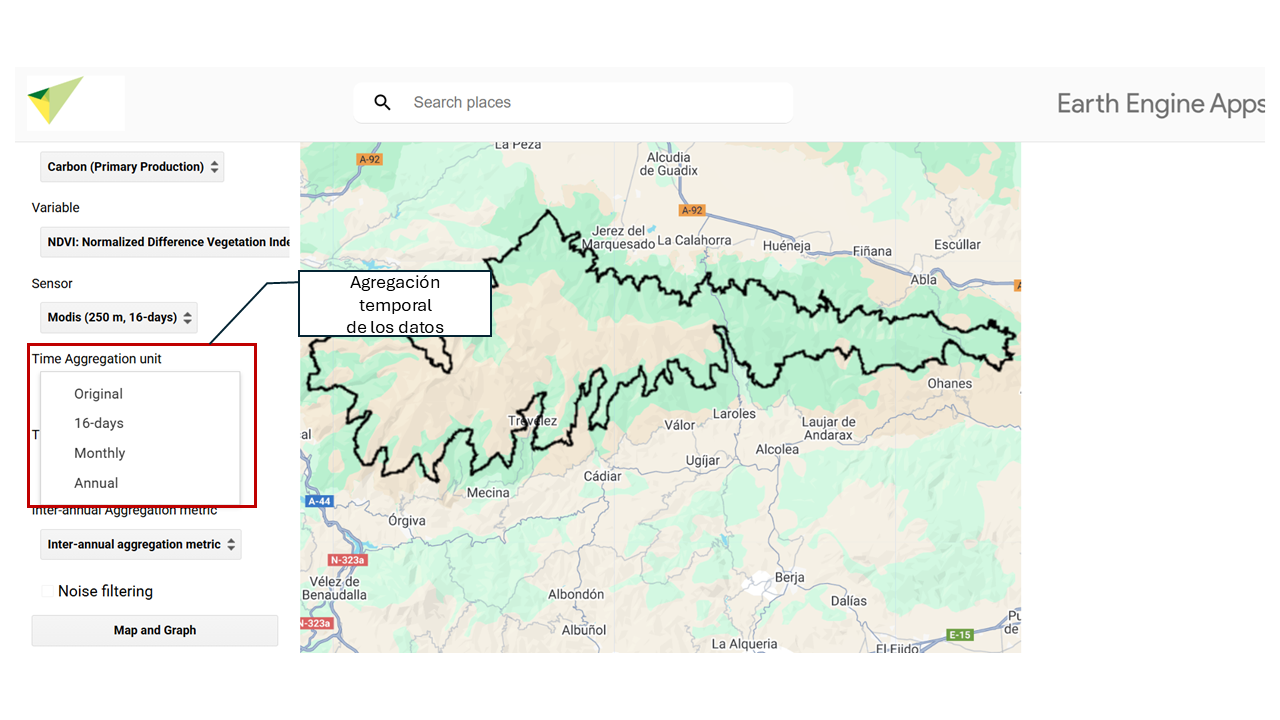
\includegraphics{assets/aggregation_es.png}

\textbf{Original}

Utiliza la frecuencia nativa del sensor (por ejemplo, diaria, 5 días, 16 días, etc.).

\textbf{Cada 16 días}

Agrupa las observaciones disponibles en intervalos de 16 días.

\textbf{Mensual}

Resume los datos por mes.

\textbf{Anual}

Genera una única observación agregada por año.

La agregación temporal permite suavizar variaciones de corto plazo, facilitar
comparaciones entre periodos, reducir la influencia de datos atípicos o evitar la
perdida de información ocasionado por la presencia de nubes en el área de interés en
fechas concretas.

\chapter{Métrica de agregación temporal}\label{agregacion-temporal}

Selecciona el \textbf{método de agregación temporal} que se aplicará al conjunto de datos. Esta opción permite \textbf{resumir series temporales} utilizando funciones estadísticas denominadas \textbf{reductores} (\emph{reducers}), entre los que se encuentran:

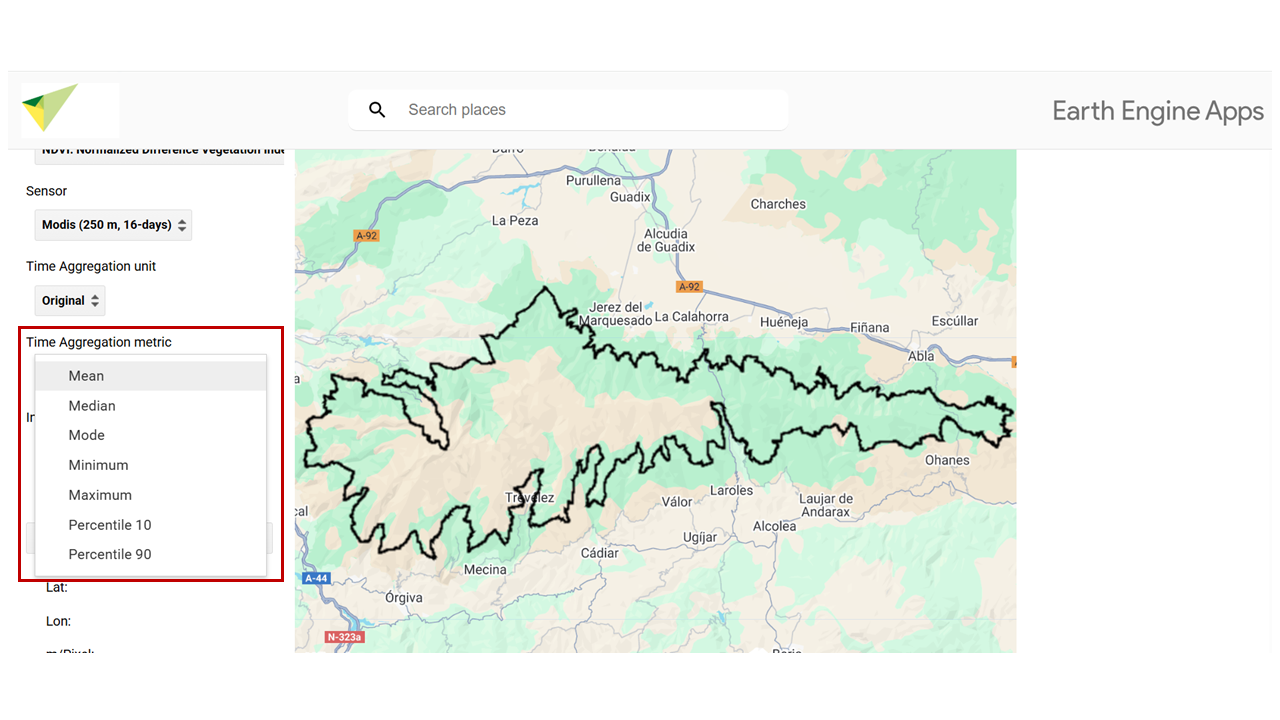
\includegraphics{assets/aggregationTime.png}

\textbf{Media}

Calcula el \textbf{promedio} de los valores dentro del período de tiempo seleccionado.

\textbf{Mediana}

Calcula el \textbf{valor central} en un conjunto de datos ordenados. Es más resistente a valores extremos que la media.

\textbf{Moda}

Calcula el \textbf{valor más frecuente} en un conjunto de datos.

\textbf{Mínimo}

Calcula el \textbf{valor más bajo} en un período de tiempo.

\textbf{Máximo}

Calcula el \textbf{valor más alto} en un período de tiempo.

\textbf{Percentil 10}

Encuentra el valor por debajo del cual está el \textbf{10\% de los datos}. Se usa para medir \textbf{valores bajos} o eventos extremos.

\textbf{Percentil 90}

Encuentra el valor por debajo del cual está el \textbf{90\% de los datos}. Se usa para medir \textbf{valores altos} o eventos extremos.

\chapter{Métrica de agregación temporal interanual}\label{agregacion-temporal-interanual}

Selecciona el método de agregación temporal para ejecutar tu análisis. Los métodos de \textbf{agregación temporal} permiten \textbf{resumir datos} en períodos de tiempo utilizando diferentes técnicas estadísticas llamadas \textbf{reductores}.

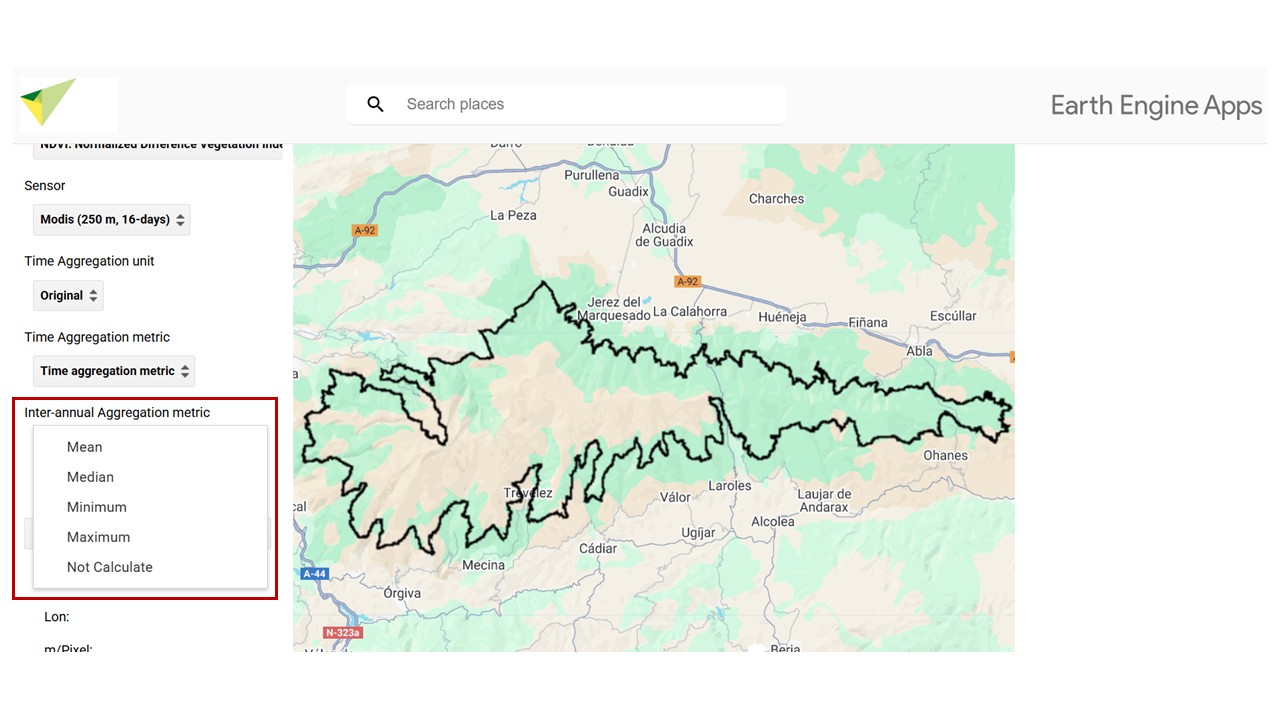
\includegraphics{assets/interannualAggregation.png}

\textbf{Media}

Calcula el \textbf{promedio} de los valores por año dentro del periodo de tiempo seleccionado.

\textbf{Mediana}

Calcula el \textbf{valor central} de los valores por año dentro del periodo de tiempo seleccionado. Es más resistente a valores extremos que la media.

\textbf{Mínimo}

Calcula el \textbf{valor más bajo} por año en un periodo de tiempo.

\textbf{Máximo}

Calcula el \textbf{valor más alto} por año en un periodo de tiempo.

\textbf{No calcular}

No calcula agregaciones temporales por años.

\chapter{Filtrado de calidad}\label{filtrado-nubes}

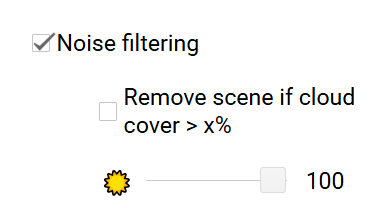
\includegraphics{assets/filter.png}

Al activar esta casilla, se aplicará un \textbf{filtrado de nubes por escena}. El filtrado de nubes por escena es un proceso utilizado en el análisis de imágenes satelitales para eliminar o reducir la interferencia causada por la presencia de nubes en cada imagen, mejorando la calidad de los datos. Como resultado, los análisis reflejarán con mayor precisión las características reales de la superficie terrestre.

Puedes establecer un \% de nubosidad, que eliminará las escenas o imágenes que superen el umbral establecido.

\chapter{Generar mapas y gráficos de resultados}\label{mapas-graficos}

\section{\texorpdfstring{\textbf{Calcular}}{Calcular}}\label{calcular}

Al hacer clic en el botón se generará el resultado según tu selección previa.

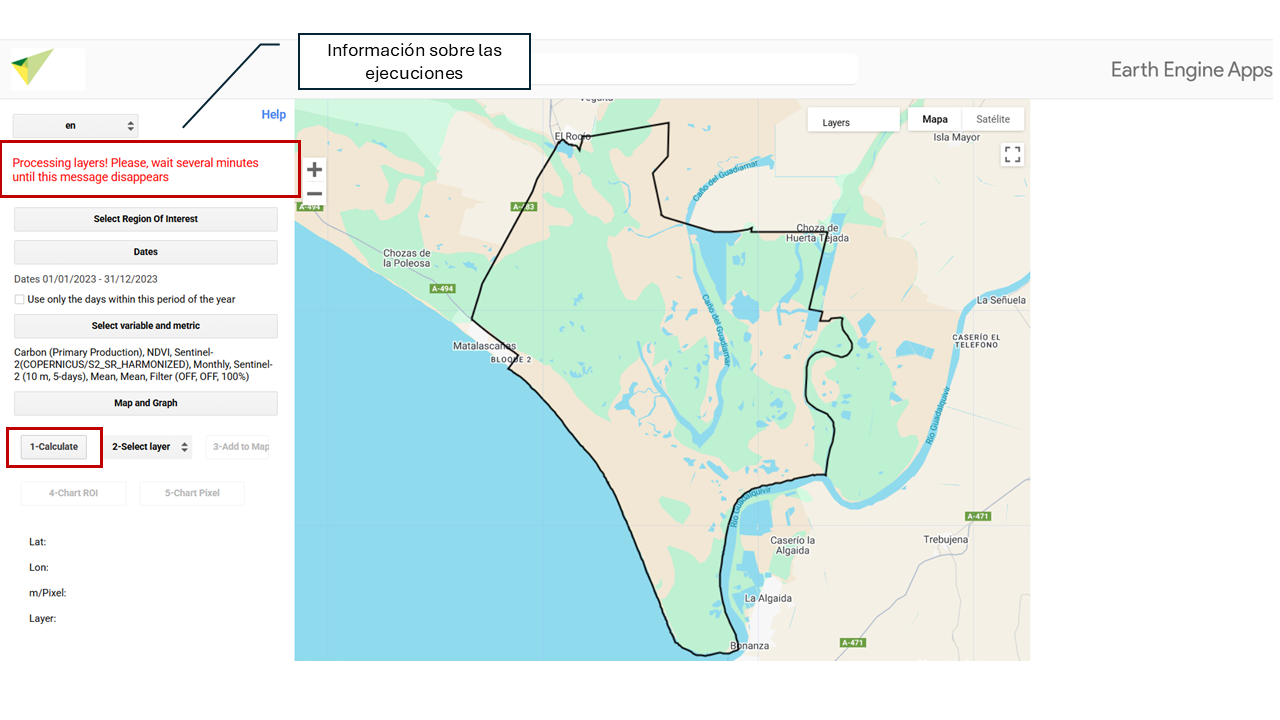
\includegraphics{assets/message_es.png}

\section{\texorpdfstring{\textbf{Seleccionar capa}}{Seleccionar capa}}\label{seleccionar-capa}

En la sección aparecerán todas las capas/mapas generados durante el cálculo. Para visualizar una capa específica, selecciónala en \textbf{``2- Seleccionar capa''} y haz clic en \textbf{``3 - Añadir al mapa''}.

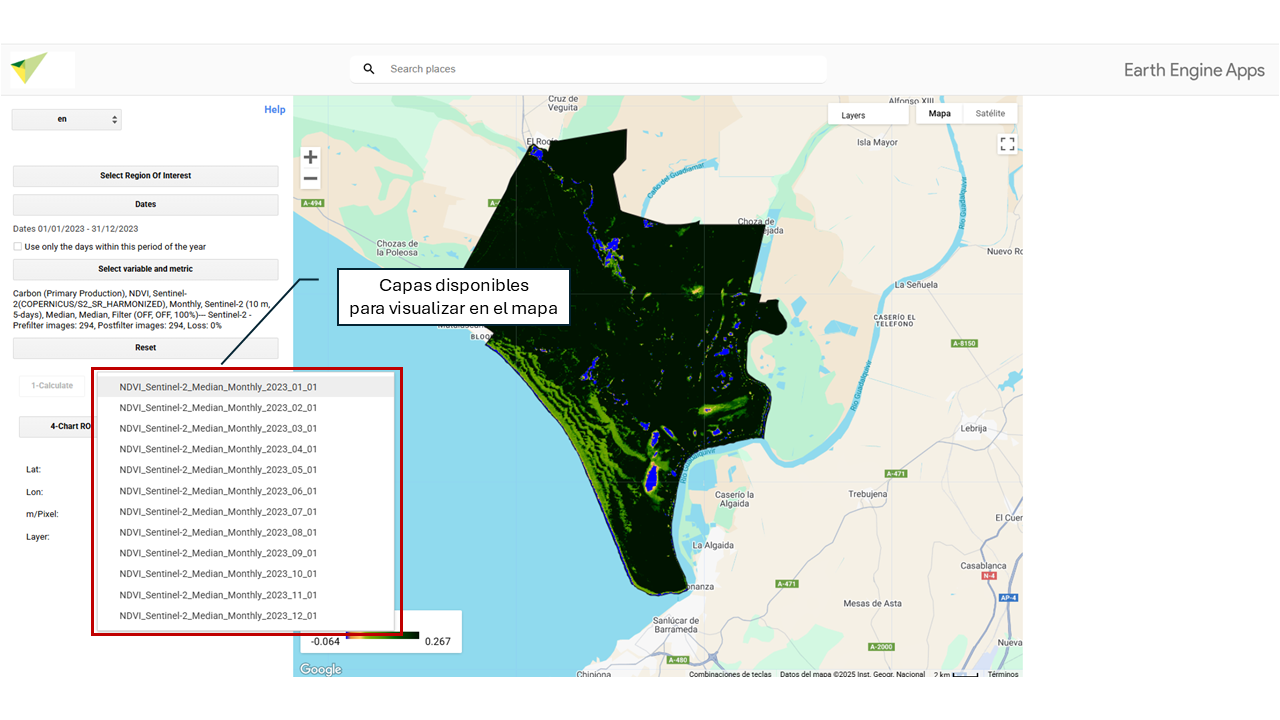
\includegraphics{assets/layers_es.png}

\section{\texorpdfstring{\textbf{Añadir al mapa}}{Añadir al mapa}}\label{auxf1adir-al-mapa}

Dibuja en el mapa la capa seleccionada.

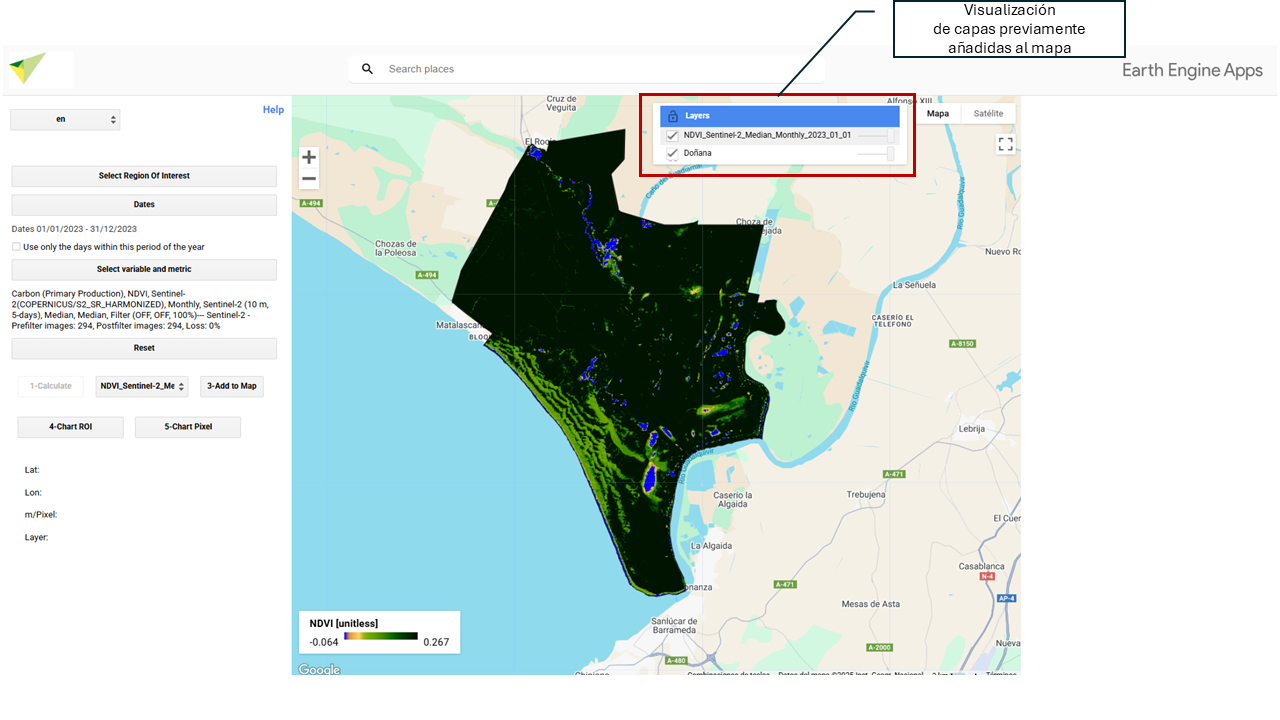
\includegraphics{assets/layers_es2.png}
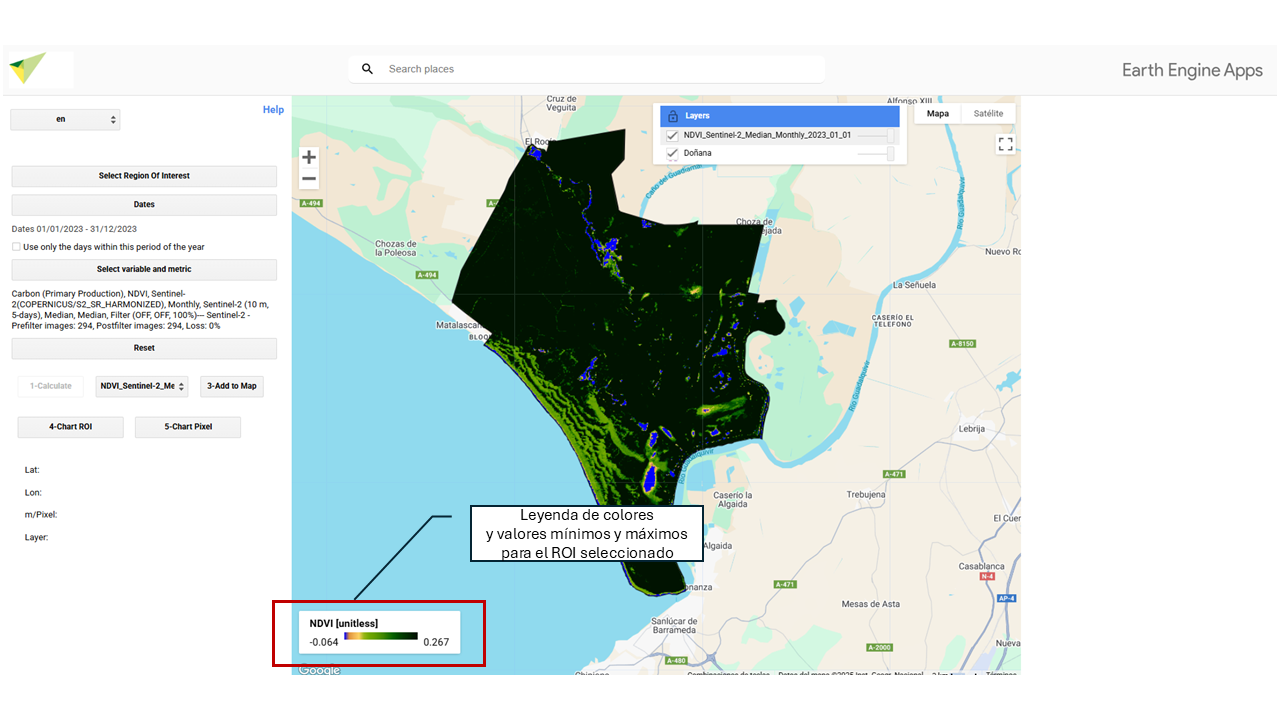
\includegraphics{assets/leyenda_es.png}

\section{\texorpdfstring{\textbf{Gráfico ROI}}{Gráfico ROI}}\label{gruxe1fico-roi}

Genera y visualiza los gráficos asociados a los mapas resultantes de tu Región de Interés (ROI por su siglas en inglés). Genera un calculo promedio.

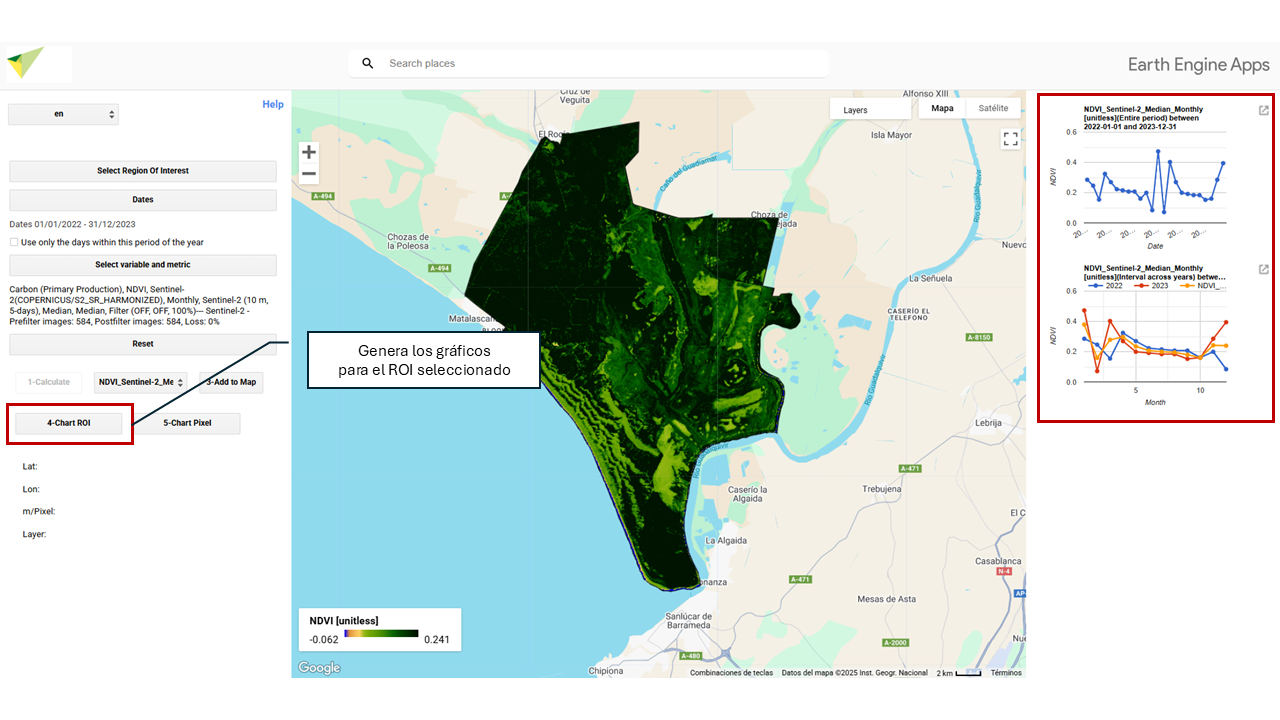
\includegraphics{assets/graphs_es.png}

\section{\texorpdfstring{\textbf{Gráfico Pixel}}{Gráfico Pixel}}\label{gruxe1fico-pixel}

Genera y visualiza los gráficos asociados a un píxel seleccionado con tu cursor. Cuando pinchas en un punto de tu área de estudio, esta opción te mostrará los datos correspondientes a su Latitud, Longitud, m/píxel (muestra la resolución del mapa en ese nivel de zoom, en metros por píxel) y el nombre de la capa que estás visualizando.

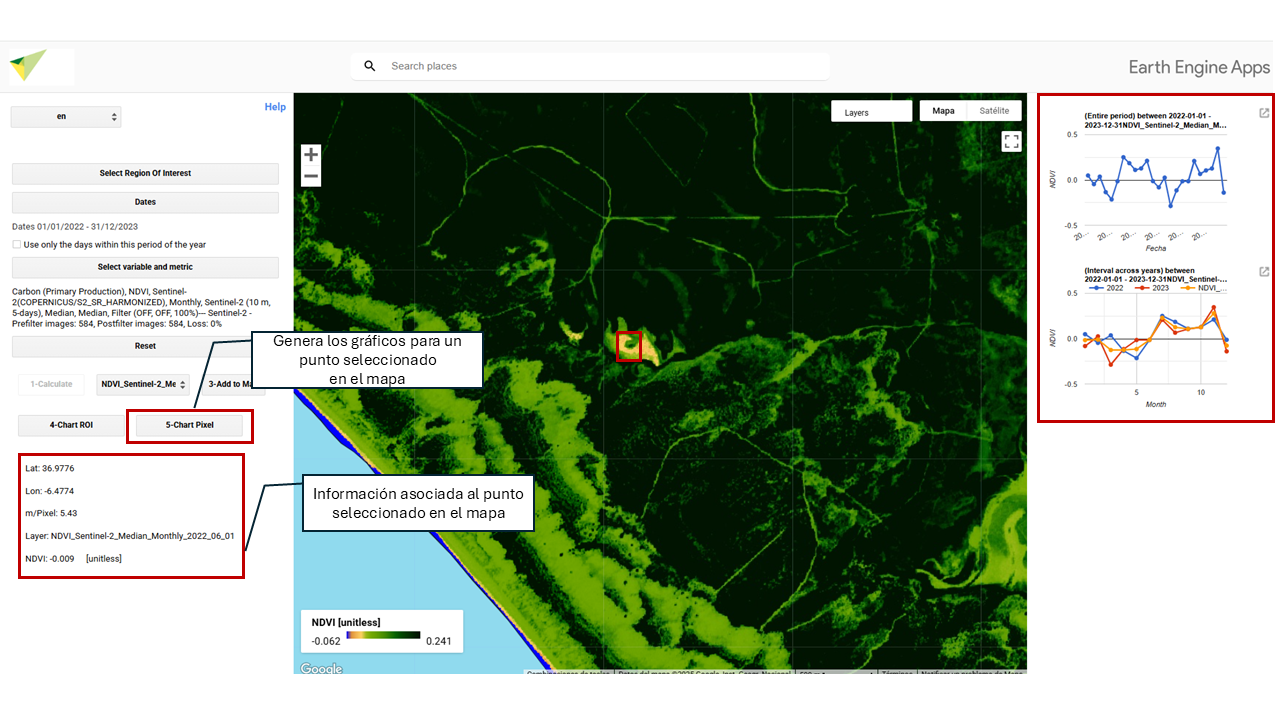
\includegraphics{assets/chart_pixel_es.png}

  \bibliography{book.bib,packages.bib}

\end{document}
